\documentclass[11pt]{article}

\usepackage{amsmath,graphicx}
\usepackage{amssymb,amsthm,bm,url,paralist,tabls,hyperref,amscd,appendix}
\usepackage{algorithm}
\usepackage[noend]{algpseudocode}


\newtheorem{thm}[equation]{Theorem}
\newtheorem{prop}[equation]{Proposition}
\newtheorem{lem}[equation]{Lemma}
\newtheorem{cor}[equation]{Corollary}
\newtheorem{conj}[equation]{Conjecture}
\newtheorem{rem}[equation]{Remark}
\newtheorem{examp}[equation]{Example}
\newtheorem{defn} [equation]{Definition}
\theoremstyle{remark}	  \newtheorem*{remark}{Remark}

\makeatletter
\def\BState{\State\hskip-\ALG@thistlm}
\makeatother

\DeclareMathOperator*{\argmin}{arg\,min}

\numberwithin{equation}{section}
\usepackage{varioref}
\labelformat{section}{Section~#1}
\labelformat{subsection}{Section~#1}
\labelformat{subsubsection}{Section~#1}
\labelformat{figure}{Figure~#1}
\labelformat{table}{Table~#1}
\labelformat{defin}{Definition~#1}
\usepackage[letterpaper,margin=1in]{geometry}

\renewcommand{\vec}[1]{\mathbf{#1}}

\title{Training Support Vector Machines with Weighted Reduced Convex Hulls}
\author{Mohammed Modan \\  Department of Mathematics, Statistics, and Computer Science \\  Macalester College \\   St. Paul, MN 55105
}



\date{December 20, 2017}

\begin{document}




\maketitle

\begin{abstract}
\noindent
Support Vector Machines have long been inaccessible for beginners beyond the linearly separable case. The geometric interpretation of SVM trainers affords a conceptually simple introduction to the subject, while still maintaining competitive accuracy and speed. In this paper, I describe the application and implementation of weighted reduced convex hulls in support vector machine classifiers. $\vec{a}$

 \end{abstract}


\section{Introduction}

Machine learning has come to run the world. From recommender systems to predictive analytics, machine learning is integrated into almost every interaction we make with technology. Machine learning can be either supervised or unsupervised. In the latter case, the algorithm is not told what to look for and discovers patterns in the data. For the former, data is preclassified and the algorithm can find patterns associated with the class provided. These algorithms, broadly, fall into either numeric predictors or classifiers. At a basic level, they operate as follows:

\begin{itemize}
	\item Train a model on input data with a known output
	\item The model can now predict an output from a new input
\end{itemize}

Algorithms can range from the relatively simple, like Naive Bayes, to the complicated and cutting edge, like neural networks. Each algorithm has its place and application in which the model will excel, and engineers/data scientists will capitalize on this fact to build their software accordingly to exploit the strengths of these algorithms. For example, Naive Bayes is frequently used for sentiment analysis or spam filtering. Support Vector Machines (SVMs) are commonly used in hand writing recognition and protein classification due to its versatility.

SVMs typically perform very well while simultaneously avoiding overfitting data. Unfortunately, SVMs come with their drawbacks as well. They may not perform as well with very noisy data, and along with other complex machine learning algorithms such as neural networks, SVMs can be difficult to interpret and they are often seen as a "black box." When explaining the algorithm is necessary for a client, simpler algorithms such as decision trees or logistic regression are typically used which are simple to interpret.

\section{What is an SVM?}

A Support Vector Machine (SVM) is indeed a type of machine learning algorithm. In order to understand their method of function, however, it is necessary to understand the format of the data. Columns of a dataset can be considered variables, and rows as observations. Each row additionally has an associated class. Each row can be viewed as a point with an associated class in ${\rm I\!R}^{v}$ where $v$ equals the number of variables. For example consider the \texttt{iris} dataset in R (\ref{table:iris}). Each row is a point in ${\rm I\!R}^{2}$.

\begin{table}[h]
\centering
\begin{tabular}{c c | c}
Petal Length  & Petal Width & Species \\
\hline
1.4 & 0.2 & setosa  \\
1.4 & 0.3 & setosa  \\
1.3 & 0.2 & setosa  \\
4.7 & 1.4 & versicolor \\
4.5 & 1.5 & versicolor \\
4.9 & 1.5 & versicolor  \\
\end{tabular}
\caption{The \texttt{iris} dataset in ${\rm I\!R}^{2}$}
\label{table:iris}
\end{table}

Notice that these points can be plotted in ${\rm I\!R}^{2}$, coloring them by an arbitrarily assigned positive or negative class. Observe that this may give rise to class separation in the Cartesian plane. As illustrated in \ref{fig:margin}, a vector $w$ can then span between convex hulls of the positive and negative classes. The margin is defined as the norm of $w$, and the hyperplane separating the hulls is the perpendicular bisector of $w$. Note that an infinite number of $w$ can be drawn to separate the data, however there exists one unique hyperplane which maximizes the margin and maximizes separation. This occurs when $w$ spans the closest points between the convex hulls, as it does in \ref{fig:margin}. This $w$ defines the maximum margin and therefore maximally separating hyperplane.

\begin{figure}[ht]
$$
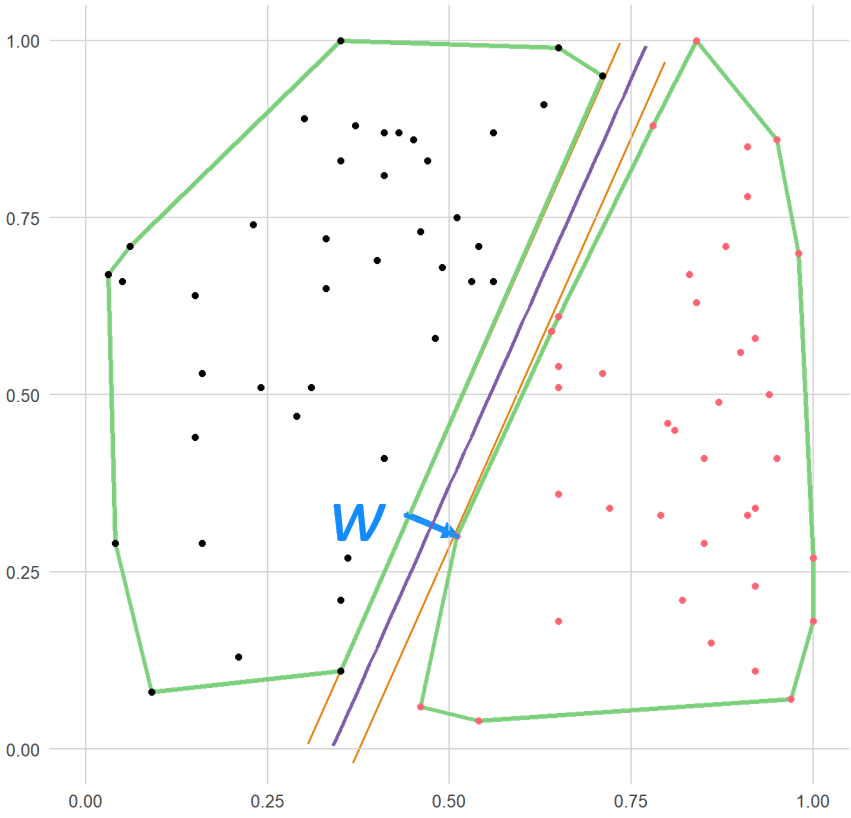
\includegraphics[width=4in]{Figs/hullPlane.PNG} 
$$
\caption{A dataset in ${\rm I\!R}^{v}$ with associated positive (salmon) and negative (black) classes. $w$ indicates the vector spanning the shortest distance between convex hulls of the classes (green), pointing to the positive class, defining the maximum margin (orange) hyperplane (purple) as its perpendicular bisector}
\label{fig:margin}
\end{figure}

Therefore we can define an SVM as follows:

\begin{defn}  An \emph{SVM} is a classifier defined by a maximally separating hyperplane.
\end{defn}

Additionally, note that once the hyperplane is found, predictions are quite simple. $w \cdot x + b < 0 $ defines the negative class, $w \cdot x + b > 0 $ defines the positive class, and $w \cdot x + b = 0$ defines the hyperplane itself.

\section{Defining the Optimization Problem}

While there are several approaches in finding the maximum margin hyperplane, we will focus on the entirely geometric approach, which relies on an iterative, interpretable algorithm. Other methods involve solve quadratic programs, which lose the geometric elegance of the solution.

First, let us mathematically outline the problem we are trying to solve. Given a set of points $P = \{x_{1}, x_{2}, ..., x_{n} | x_{i}\in{\rm I\!R}^{d}\}$ and their associated labels $Y = \{y_{1}, y_{2}, ..., y_{n} | y_{i}\in \{1,-1\}\}$, we can write the equation of the convex hull as:

\begin{equation}
CH(P) = \Bigg \lbrace \sum_{i=1}^{n} \alpha_{i}x_{i} \;\;\; \Bigg \vert \;\;\; x_{i} \in P,\;\; \sum_{i=1}^{n} \alpha_{i} = 1,\;\; 0 \leq \alpha_{i} \leq 1 \Bigg \rbrace
\end{equation}

Where finding the maximum margin is equivalent to solving the minimization task given by \ref{minim} and \ref{subto} \cite{theodoridis_reduced_2007}.

\begin{equation}
\textrm{minimize} \quad \sum_{i,j} y_{i}y_{j} \alpha_{i} \alpha_{j} \mathbf{x_{i}^{T} x_{j}},
\label{minim}
\end{equation}
\begin{equation}
\textrm{subject to} \quad \sum_{i=1}^{n} \alpha_{i}y_{i} = 0, \;\; \sum_{i=1}^{n} \alpha_{i}=2, \;\; \alpha_{i} \geq 0
\label{subto}
\end{equation}

An iterative algorithm to find this optimal solution was found by Kozinec, and later improved by Schlesinger to converge at an $\epsilon$-optimal solution for time efficiency \cite{franc_iterative_2003}.

\section{The Schlesinger-Kozinec Algorithm}

The Schlesinger-Kozinec (SK) algorithm maintains the geometric view of SVMs, converges very fast, and scales incredibly well \cite{goodrich_training_2011}. With this iterative approach, the algorithm essentially needs to "check" points on the convex hulls, but does not actually have to compute the entire hull. This allows the algorithm to rapidly scale to higher dimensions without increasing time complexity. This efficient aspect of the algorithm relies on a \texttt{findVertex} function, as outlined in Algorithm \ref{alg:findVert} and in \ref{fig:findVert}. This algorithm will find the point on the CH of $P$ in the direction of $\mathbf{n}$.

\begin{algorithm}
\caption{Finding a CH vertex}\label{euclid}
\begin{algorithmic}[1]
\Function{findVertex}{$P, \mathbf{n}$}
    \State $a \gets \argmin_{i} \{\mathbf{n \cdot x_{i}} \}$
    \State \Return $\mathbf{x_{i}}$
\EndFunction
\end{algorithmic}
\label{alg:findVert}
\end{algorithm}

\begin{figure}[h]
$$
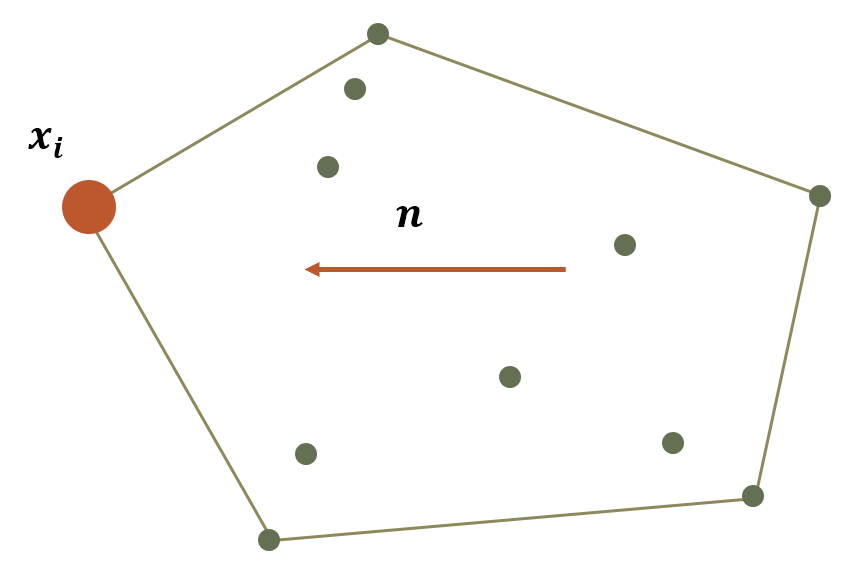
\includegraphics[width=3in]{Figs/findVertex.png}
$$
\caption{the findVertex routine will find the vertex $x_{i}$ on the convex hull of $P$ in the direction of $\mathbf{n}$}
\label{fig:findVert}
\end{figure}

Now, given a positive and negative point set, we can work with two candidate nearest points, $\mathbf{p_{pos}}$ and $\mathbf{p_{neg}}$, we can find $w$ as equation \ref{eqn:w}.

\begin{equation}
w = p_{pos}-p_{neg}
\label{eqn:w}
\end{equation}

With each iteration of the algorithm, the candidate points will move closer and closer to the true closest points of the convex hulls, eventually defining the optimal $\mathbf{w}$ and hyperplane.

\subsection{Initialization}

Thanks to Goodrich \cite{goodrich_training_2011}, a thorough understanding of this algorithm has been made possible. While Goodrich initializes $p_{pos}$ and $p_{neg}$ as any random point on their respective hulls, I found this to lead to wildly inconsistent training times. Instead, I propose initialization based on the centroids of each point set, which can be calculated by averaging all points. Thereafter, $p_{pos}$ can be initialized as $\texttt{findVertex}(center_{neg} - center_{pos})$ and $p_{neg}$ can be initialized as $\texttt{findVertex}(center_{pos} - center_{neg})$. This ensures that the starting points will at least initialize on at least the correct half of the convex hulls.

Additionally, update vertices $v_{pos}$ and $v_{neg}$ are initialized as $\texttt{findVertex}(-w)$ and $\texttt{findVertex}(w)$ respectively. These will be used to updated $p_{pos}$ and $p_{neg}$.

\subsection{Stopping Conditions}

If the new $v_{pos}$ and $v_{neg}$ are within $\epsilon$ to $p_{pos}$ and $p_{neg}$, the algorithm is terminated. This is checked confirming that both \ref{eqn:stop1} and \ref{eqn:stop2} are satisfied.

\begin{equation}
1-\frac{w \cdot (v_{pos}-p_{neg})}{||w||^{2}} < \epsilon
\label{eqn:stop1}
\end{equation}
\begin{equation}
\texttt{and} \quad 1-\frac{w \cdot (v_{neg}-p_{pos})}{||w||^{2}} < \epsilon
\label{eqn:stop2}
\end{equation}

Essentially, $\epsilon$ optimality is reached with the w created by the update vertex and the old candidate is close enough to $w$ created by the candidate points.

\subsection{Adaptation}

First, choose to either update the positive or negative class. If $w \cdot (p_{pos} - v_{pos}) > w \cdot (p_{neg} - v_{neg})$, then there is more room for potential progress to be made on the positive hull so $p_{pos}$ is updated. Otherwise, $p_{neg}$ is updated.

$p_{pos}$ is updated by finding the point on the line segment created by $p_{pos}$ and $v_{pos}$ that is closest to $p_{neg}$. This happens to be at the point where $w$ is orthogonal to $p_{pos}-v_{pos}$ and connects via $p_{neg}$. This is graphically illustrated in \ref{fig:updateFig}. $p_{pos}^{new}$ can then be found from Equation \ref{eqn:newp}.

\begin{equation}
p_{pos}^{new} = (1-q)p_{pos}+q v_{pos}\;, \quad q\in[0,1]
\label{eqn:newp}
\end{equation}

Where $q$ is found such that $w^{new} \cdot (p_{pos}-v_{pos}) = 0$ to ensure they are orthogonal. $q$ is clamped between 0 and 1 to ensure the new point lies between the candidate and update points. Substituting \ref{eqn:newp} and $p_{neg}$ for $w^{new}$ gives rise to Equation \ref{eqn:orthog} where $q$ can be solved for to yield \ref{eqn:posupdate}.

\begin{equation}
0 = \bigg(p_{neg} - ((1-q)p_{pos}+q v_{pos})\bigg) \cdot \bigg(p_{pos}-v_{pos}\bigg)
\label{eqn:orthog}
\end{equation}
\begin{equation}
q=\frac{(p_{pos}-p_{neg}) \cdot (p_{pos}-v_{pos})}{(p_{pos}-v_{pos})^{2}}
\label{eqn:posupdate}
\end{equation}

$p_{neg}$ is updated similarly, with Equations \ref{eqn:orthogneg} and \ref{eqn:negupdate}.

\begin{equation}
p_{neg}^{new} = (1-q)p_{neg}+q v_{neg}\;, \quad q\in[0,1]
\label{eqn:orthogneg}
\end{equation}
\begin{equation}
q=-\frac{(p_{pos}-p_{neg}) \cdot (p_{neg}-v_{neg})}{(p_{neg}-v_{neg})^{2}}
\label{eqn:negupdate}
\end{equation}

\begin{figure}[h]
$$
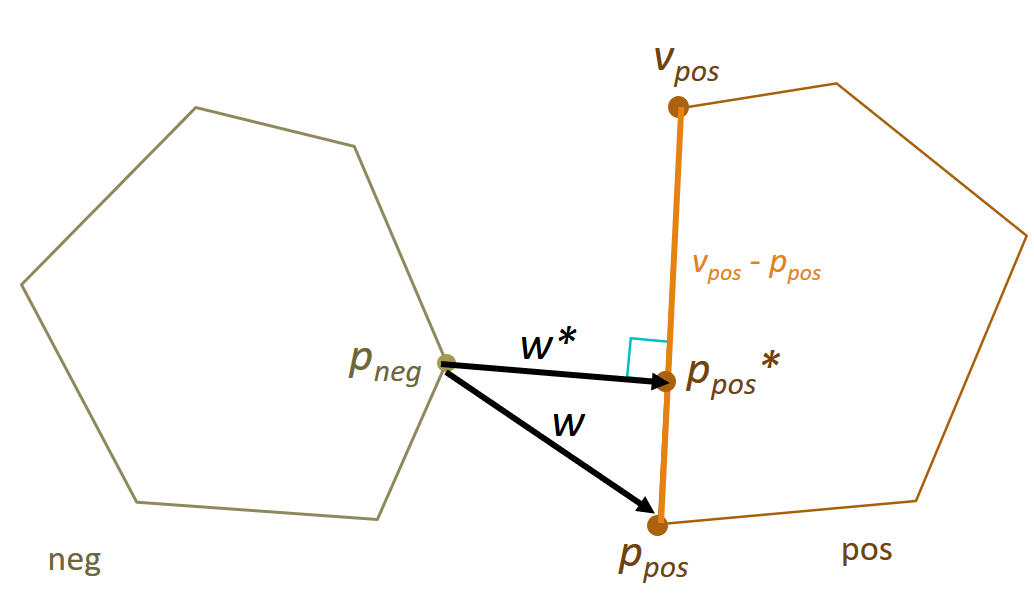
\includegraphics[width=4in]{Figs/update.PNG}
$$
\caption{A new $p_{pos}$ is found such that it minimizes distance to $p_{neg}$. This requires that the new $w$ be orthogonal to $p_{pos}-v_{pos}$.}
\label{fig:updateFig}
\end{figure}

\section{Weighted Convex Hull Reduction}
Notice that up to now, only the linearly separable case has been considered for points set. However, most data cannot be linearly separated. To maintain the geometric beauty of the algorithm, consider a reduction of the convex hull for each class. In addition, consider that it would be possible to reduce the convex hull based on the weight of each point.

Franc and Hlavac \cite{franc_iterative_2003} explored this idea and adapted the SK algorithm accordingly. In addition, Goodrich \cite{goodrich_training_2011} introduced individual point weights to the SK algorithm. In fact, the algorithm remains the same, only the \texttt{findVertex} function changes to account for the new type of hull, taking in two new parameters as well: $\mu$ and $s$, corresponding to the reduction factor and weights respectively. The new \texttt{findVertex} is discussed further in \cite{goodrich_training_2011}. For my implementation, the centroids of the hulls are now weighted averages of each point.

For a weighted reduced convex hull (WRCH), the definition changes only slightly to yield Equation \ref{wrch}

\begin{equation}
WRCH(P,s,\mu) = \Bigg \lbrace \sum_{i=1}^{n} \alpha_{i}x_{i} \;\;\; \Bigg \vert \;\;\; x_{i} \in P,\;\; \sum_{i=1}^{n} \alpha_{i} = 1,\;\; 0 \leq \alpha_{i} \leq s_{i}\mu \Bigg \rbrace
\label{wrch}
\end{equation}

Here, $s \in {\rm I\!R}^{n}$, a vector of weights for each point. All that has changed is the upper bound on $\alpha_{i}$ to be reduced by a constant and weight. The minimization problem then becomes:

\begin{equation}
\textrm{minimize} \quad \sum_{i,j} y_{i}y_{j} \alpha_{i} \alpha_{j} \mathbf{x_{i}^{T} x_{j}},
\end{equation}
\begin{equation}
\textrm{subject to} \quad \sum_{i=1}^{n} \alpha_{i}y_{i} = 0, \;\; \sum_{i=1}^{n} \alpha_{i}=2, \;\; 0 \leq \alpha_{i} \leq s_{i}\mu
\end{equation}

This new minimization problem allows for linear separability that can also account for weighted points, as demonstrated in \ref{reduction}.

\begin{figure}
$$
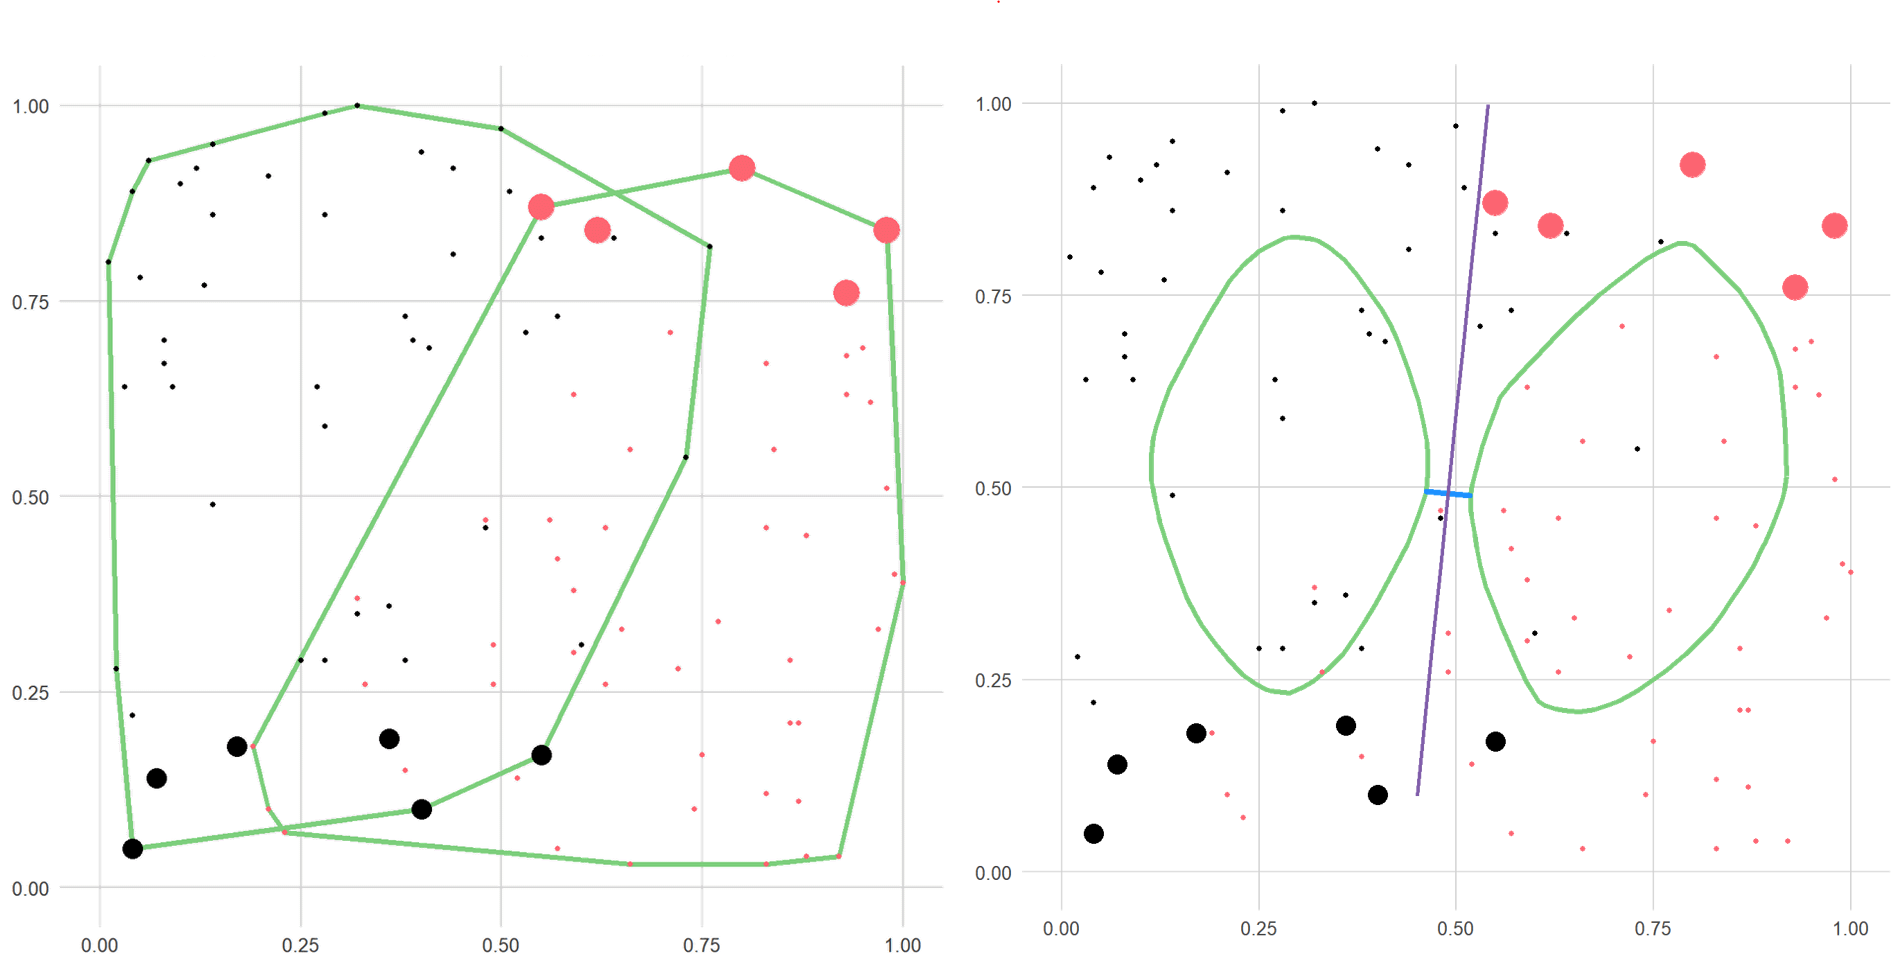
\includegraphics[width=4in]{Figs/linsep.PNG}
$$
\caption{Left: $\mu = 1$, non-linearly separable hulls. Right: Weighted reduction to $\mu = 1/30$. Linearly separable hulls, SK proceeds as normal}
\label{reduction}
\end{figure}

\section{Tests}
After implementing the weighted SK algorithm described by Goodrich \cite{goodrich_training_2011}, I tested the data on two datasets from the UCI machine learning repository after normalization - \texttt{wine} and \texttt{heart}. Classifying wine 1 from wines 2 and 3 from alcohol content, flavinoid content, and magnesium content yielded an astonishing 94.3\% accuracy, completing in just 5 iterations, very quick considering each loop runs  with O(n) time complexity.

A preliminary test on the \texttt{heart} dataset, considering all variables, yielded 77.4\% accuracy in predicting which patients had heart disease, but 13\% of cases were false negatives. To remedy this, weighing the positive for disease class 5x more increased accuracy to 78.5\% and decreased false negatives to only 3\%.

It is important to note that for all tests,$\epsilon$ can vary depending on the required accuracy, but as per instructions in Goodrich \cite{goodrich_training_2011}, $\mu=\frac{1}{0.9\kappa}$ where $\kappa =$ the sum of weights in the smallest by weight class. This leads to a 90\% hull reduction in the smallest class, guaranteeing separability. Goodrich did not elaborate on why or how this guarantees separability and I have not been able to reach a conclusion.

\section{Conclusion and Future}

A conceptually simple, geometric interpretation of SVM training allows for more accessibility. We have seen how the geometric algorithm for convex hulls can be adapted for reduced convex hulls as well, with high accuracy.

For future work, I hope to transfer computations to Java for speed, expand to a multiclass SVM, and implement kernels to afford greater accuracy and adaptability.

\bibliography{ExportedItems}
\bibliographystyle{ieeetr}
\end{document}